%AAAAAAAAAAAAAAAAAAAAAAAAAAAAAAAAAAAAAAAAAAAAAAAAAAAAAAAAAAAAAAAAAAAAAAAAAAAAAAAAAAAAAAAAAAAAAAAAAAAAAAAAAAAAAAA
%AAAAAAAAAAAAAAAAAAAAAAAAAAAAAAAAAAAAAAAAAAAAAAAAAAAAAAAAAAAAAAAAAAAAAAAAAAAAAAAAAAAAAAAAAAAAAAAAAAAAAAAAAAAAAAA

%Ce document est r�alis� par
%Mlle S. BOUCHELAGHEM Doctorante/Enseignante
%D�partement d'Informatique, Universit� de B�jaia

%Pour les �tudiants de Licence 3 en Informatique
%Dans le cadre du module *** R�daction Scientifique ***

% ***Avril 2018***

%AAAAAAAAAAAAAAAAAAAAAAAAAAAAAAAAAAAAAAAAAAAAAAAAAAAAAAAAAAAAAAAAAAAAAAAAAAAAAAAAAAAAAAAAAAAAAAAAAAAAAAAAAAAAAAA
%AAAAAAAAAAAAAAAAAAAAAAAAAAAAAAAAAAAAAAAAAAAAAAAAAAAAAAAAAAAAAAAAAAAAAAAAAAAAAAAAAAAAAAAAAAAAAAAAAAAAAAAAAAAAAAA

\documentclass[12pt]{report}
\usepackage[latin1]{inputenc}
\usepackage[T1]{fontenc}
\usepackage[francais]{babel}
\usepackage{graphicx}
\usepackage{layout}
\usepackage[top=2cm, bottom=2cm, left=2cm, right=2cm]{geometry}
\usepackage{url}
\usepackage{fancyhdr}
\usepackage{color}
\usepackage{colortbl}
\usepackage{multirow}
\usepackage{nomencl}
\usepackage{setspace}


\makenomenclature

\definecolor{lightgray}{gray}{0.85}
\pagestyle{fancy}

\fancyhead[L]{}

\begin{document} 

%%%% Page de garde %%%%
%%%%%%%%%%%%%%%%%%%%%%%
%%%% Page de garde %%%%
%%%%%%%%%%%%%%%%%%%%%%%

\begin{titlepage}

\begin{center}

  \large{R�publique Alg�rienne D�mocratique et Populaire}\\
  \large{Minist�re de l'Enseignement Sup�rieur et de la Recherche Scientifique}\\
  \large{Universit� A. Mira de B�ja�a}\\
  \large{Facult� des Sciences Exactes}\\
  \large{D�partement d'Informatique}\\


	\begin{figure}[h!]
		\centering
		\includegraphics[width=6cm]{images/logo.jpg}
	\end{figure}
	
    \paragraph{}
     
		{\LARGE{\textbf M�moire de Fin de Cycle}} \\[2ex]
    \textbf En vue de l'obtention du dipl�me de Licence en Informatique G�n�rale \\[1ex]
    \paragraph{}
		
    \textbf{Th�me}\\[1ex]
		\rule{\textwidth}{1pt}
        {\LARGE{\textbf{{\\
    Conception et r�alisation d'une application Android pour la gestion du temps de l'�tudiant \\}}}}
		\rule{\textwidth}{1pt}\\
	  \vspace{0.2cm}

\end{center}

\begin{center}

\large R�alis� par

\paragraph{}

\begin{tabular}{l l l l}	

		M. TAYEB CHERIF Mohand Said 					& & & 		M. SALIMI Salim \\
								
		M. YAYADENE Abderzak 		& & & 		M. ZADIR Azzedine \\		
		
		
\end{tabular}
		
\paragraph{}

 Devant le jury compos� de

\end{center}
  
\paragraph{}
  
\begin{table}[h!]
\begin{center}
        \begin{tabular}{l l l}
				\textbf{Pr�sidente :} & M$^{me}$ F. BOULAHROUZ & Universit� de B�ja�a \\
				
				\textbf{Examinateur :} & M. M. MOKTEFI  &  Universit� de B�ja�a \\
				
				\textbf{Encadrant :} & M. K. AKILAL  & Universit� de B�ja�a \\
				
        \end{tabular}    
\end{center}

\end{table}

\begin{center} Promotion 2017 - 2018 \end{center}


\end{titlepage}


%%%% Remerciements %%%%
\begin{titlepage}
\newpage
\pagestyle{fancy}      
\lhead{}  
\chead{}     
\rhead{}     
    
\renewcommand{\headrulewidth}{0.5pt}

\chapter*{\hrulefill ~~\textbf{Remerciements}~ \hrulefill}
\paragraph{}
\paragraph{}
\large

	  \textbf{P}our commencer, nous tenons \`a remercier notre encadrant M. K. AKILAL, pour l'orientation, la confiance, la patience qui ont constitu\'e un apport consid\'erable sans lequel ce travail n'aurait pas pu \^etre men\'e \`a bon port. 
		
		\paragraph{}
			
		\textbf{N}os remerciements s'\'etendent \'egalement \`a M$^{lle}$ S. BOUCHELAGHEM pour le pr\'ecieux temps qu'elle nous a consacr\'e, aux personnes qui nous ont apport\'e leur aide pr\'ecieuse et qui ont contribu\'e \`a l'\'elaboration de ce travail.
		
		\paragraph{}
		
		\textbf{N}ous remercions \'egalement chacun des membres du jury pour l'int\'er\^et qu'ils ont port\'e pour notre travail, pour les remarques et les conseils contribuant ainsi \`a l'enrichissement de ce modeste travail.
		
		\paragraph{}
		\textbf{E}nfin, nous adressons nos plus sinc\`eres remerciements \`a nos familles, \`a nos proches et \`a nos amis, qui nous ont accompagn\'e, aid\'e, soutenu et encourag\'e tout au long de la r\'ealisation de ce m\'emoire. 
		
		\paragraph{}
		
		
		
		\paragraph{}
		


\thispagestyle{empty}		

\end{titlepage}	

%%%% D�dicaces %%%%
\input{D�dicaces}

%D�but de la num�rotation romaine pour la table des mati�res
\newpage 
\pagenumbering{roman}

%Construire la table des mati�res
\addcontentsline{toc}{part}{Table des mati�res} 
\tableofcontents
\fancyhead[R]{}
\renewcommand{\headrulewidth}{0pt}

%Construire la table des figures
\listoffigures
\addcontentsline{toc}{part}{Table des figures}

%Construire la liste des tableaux
\listoftables
\addcontentsline{toc}{part}{Liste des tableaux}

%Construire la liste des abr�viations
\nomenclature{\textbf{UML}}{Unified Modeling Language}
\nomenclature{\textbf{SE}}{Syst�me d'Exploitation}
\nomenclature{\textbf{IHM}}{Interactions homme-machine}
\nomenclature{\textbf{HTML}}{HyperText Markup Language }
\nomenclature{\textbf{CSS}}{Cascading Style Sheets }
\nomenclature{\textbf{iOS}}{iPhone Operating System }
\nomenclature{\textbf{SDK}}{Software Developpement Kit }
\nomenclature{\textbf{JDK}}{Java Developement Kit}
\nomenclature{\textbf{JVM}}{Java Virtual Machine }
\nomenclature{\textbf{XML}}{Extensible Markup Language }
\nomenclature{\textbf{SQL}}{Structured Query Language}
\nomenclature{\textbf{DAO}}{Data Access Objects }
\nomenclature{\textbf{SGBD}}{Syst�me de Gestion de Base de Donn�es}
\nomenclature{\textbf{DCP}}{Diagramme de Classe Participante}
\nomenclature{\textbf{EDI}}{Environnement de D�veloppement Int�gr�}
\nomenclature{\textbf{GPL}}{General Public License}




\def\nomname{Liste des abr�viations}
\printnomenclature[2in] 
\addcontentsline{toc}{part}{Liste des abr�viations}
\fancyhead[R]{\textit{Liste des abr�viations}}
\renewcommand{\headrulewidth}{1pt}


%D�but de la num�rotation arabe pour le reste du m�moire
\newpage
\pagenumbering{arabic}

%%%% Mise en forme des titres des chapitres %%%%
\makeatletter
\def\@makechapterhead#1{%
  \vspace*{10\p@}%
  {\parindent \z@ \centering \normalfont
    \ifnum \c@secnumdepth >\m@ne
        \huge\bfseries \@chapapp\space \thechapter
        \par\nobreak
        \vskip 20\p@
    \fi
    \interlinepenalty\@M
    \Huge \bfseries #1\par\nobreak
    \vskip 40\p@
  }}
 
\def\@makeschapterhead#1{%
  \vspace*{10\p@}%
  {\parindent \z@ \centering
    \normalfont
    \interlinepenalty\@M
    \Huge \bfseries  #1\par\nobreak
    \vskip 40\p@
  }}
\makeatother 

%%%% Profondeur des sous-titres jusqu'� 4 chiffres %%%%
\setcounter{secnumdepth}{3}

%%%% Introduction G�n�rale %%%%
\input{Introduction_G�n�rale}

%%%% Chapitre 1 %%%%
\chapter{Contexte et probl�matique}
\fancyhead[R]{\textit{Contexte et probl�matique}}
\renewcommand{\headrulewidth}{1pt}


\section{Introduction}
Dans ce chapitre nous allons pr�senter en premier lieu le contexte du projet ainsi qu'une br�ve description de la probl�matique. Nous allons par la suite,pr�senter  le  langage UML et aborderons quelques d�finitions sur les applications mobile. Enfin, on termine ce premier chapitre avec l'�laboration du cahier des charges permettant d'avoir une vue globale sur les objectifs du projet.




\section{Contexte du projet}

On dit toujours que le temps est la chose la plus pr�cieuse car on peut tout acheter sauf le temps. Quoi qu'on fasse, une journ�e durera toujours 24 heures et le rythme de vie de la soci�t� moderne nous fait sentir que l'on est 
perp�tuellement en manque de temps. L'�tudiant est l'une des classes sociales les plus touch�es par ce probl�me. Entre  ses �tudes, ses activit�s sportives, ses loisirs et �ventuellement son travail a mis temps . Ainsi, il est difficile pour lui de pouvoir g�rer toutes ses t�ches quotidiennes et se retrouve parfois d�bord�.//

Les smartphones ont r�volutionn� le monde de par le nombre de fonctionnalit�s et de possibilit�s qu'ils offrent, il est de nos jours indispensable d'en poss�der dans la soci�t� moderne, plus de 50\% de la population mondial poss�de d�j� une smartphone et l'�tudiant en repr�sente une majeure partie .
  




\section{Probl�matique}
 dans ce projet nous avons d�cide de r�aliser une application mobile pour la gestion du temps de l��tudiant .elle sera capable de fournir une repr�sentation  simple et compr�hensible de l�emploi du temps comme les s�ances de cours et de travaux diriger ainsi que ses diff�rentes activit�s . elle devras aussi l'assist� au quotidien en lui rappant toutes les taches que il a pr�vue.
  
L'�tudiant a tendance � arriver en retard ou carr�ment � rater ses rendez-vous car il a pr�vu autre chose au m�me moment sans le savoir ? L'�tudiant fait pleins d'activit�s et n'arrive plus � se situer ? Il ne sait pas quoi r�pondre quand on lui demande s'il est libre � tels moment?. gr�ce a notre application nous esp�rons contribuer a r�soudre ses probl�mes afin que l��tudiant soit plus productif et mieux organiser .

Tout au long de ce travail, nous allons raisonn� avec le principe du rasoir d'Ockham �galement appel� principe de simplicit�. Vous allez voir une conception simple, des diagrammes  tr�s l�gers pour aboutir a un r�sultat fid�le � ce principe .


\section{UML}

UML (Unified Modeling Language) se d�finit comme un langage de mod�lisation graphique et textuel. Il est destin� � d�crire des besoins, sp�cifier et documenter des syst�mes, esquisser des architectures logicielles, concevoir des solutions et communiquer des points de vue. UML unifie �galement les notations n�cessaires aux diff�rentes activit�s d'un processus de d�veloppement d'applications et offre, par ce biais, le moyen d'�tablir le suivi des d�cisions prises, depuis l'expression des besoins jusqu'� l'�tape de r�alisation.\cite{1}

\begin{paragraph}
En fait, et comme son nom l'indique, UML n'a pas l'ambition d'�tre exactement une m�thode : c'est un langage. UML est donc non seulement un outil int�ressant, mais une norme qui s'impose en technologie � objets et � la quelle se sont rang�s tous les grands acteurs du domaine, acteurs qui ont d'ailleurs contribu� � son �laboration. \cite{2}
\end{paragraph}

\section{Application mobile}
Une application mobile n'est rien d'autre qu'un logiciel t�l�chargeable que l'on installe facilement sur nos smartphones(mobile intelligent) comme on ferait sur notre ordinateur. Le t�l�chargement de l'application mobile se fait suivant deux options:
\begin{itemize}
	\item Sur t�l�phone par le biais de connexion Internet.
	\item Sur ordinateur en le branchant avec le t�l�phone mobile.
\end{itemize}

Il existe trois types distincts selon leurs sp�cificit�s techniques qui sont:
\begin{description}


	
\item [Application Native : ]Ces applications sont li�s au syst�me d'exploitation sur le quel sont install�es car elles utilisent des caract�ristiques reli�es � celui-ci. Elle sont �crites dans un langage adapt� au syst�me d'exploitation en question. Ce type d'application est accessible seulement sur les syst�mes d'exploitation auxquelles sont destin�es. Ces plate-formes retirent 25\% du prix de vente pour une application native payante.
\item [Application Web :] Ce sont toutes les applications con�ues gr�ce aux outils de d�veloppent web actuels (HTML, CSS, JavaScript..). Elles sont accessible sur tout les mobiles via un navigateur Web ce qui la rend plus int�ressante sur le point de vue financier car les co�ts de d�veloppement sont r�duits vue qu'on d�veloppe une seule application qui est compatible avec tous les smartphones  quelque soit leur syst�me. 
\item[Application Hybride:] sont des applications qui incorporent les deux principes de d�veloppement des types pr�c�demment cit�s. Les caract�ristiques des applications web et celles des application native. Elles pourront �tre distribu�es sur les plate-formes de t�l�chargement telles que l'Apple Store (iOS), Play Store (Android) ou encore Windows Store (Windows Phone). L'utilisateur peut donc installer ces applications et consulter leur contenu sans avoir � passer par un navigateur web. Ce type d'application mobile minimise les charges et la dur�e de son d�veloppement m�me si cela sera au d�triment du perfectionnement et de la qualit� qui caract�rise l'application native.
\end{description}
La figure suivante illustre les trois types cit�s.
\begin{figure}[h!]
	\centering
		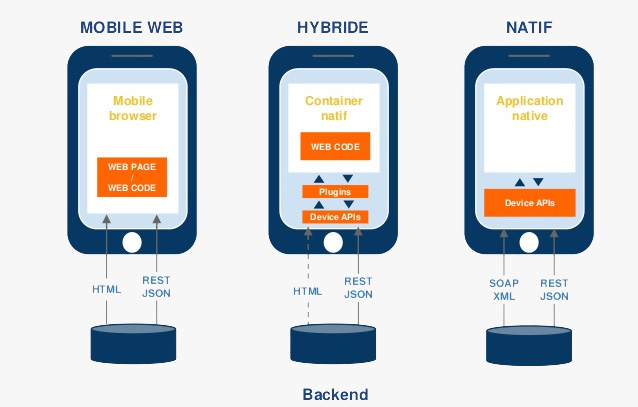
\includegraphics[width=8cm]{images/types-d-application-mobile.jpg}
	\caption{Les diff�rents types d'applications.}
	\label{typedapplication}
\end{figure}



\section{Cahier des charges}
L'application � d�velopper aura pour mission d'offrir une repr�sentation des �v�nements et des activit�s de l'utilisateur pendant les jours de la semaine. Pour cela, l'application devra r�pondre � ces besoins avec les fonctionnalit�s suivantes:
\begin{itemize}
\item Permettre � l'utilisateur d'organiser ses activit�s et les regrouper dans de diff�rents calendriers.
\item Permettre � l'utilisateur d'ajouter des activit�s dans le calendrier qui leur convient.
\item Offrir une interface intuitive � l'utilisateur pour afficher ses activit�s.
\item G�n�rer des alertes/notifications pour les activit�s correspondantes. 
\end{itemize}
 

   
\section{Conclusion}
Dans ce premier chapitre, nous avons presenter le contexte et la problematique aborder dans ce projet,defint le language uml et les application mobile et rediger un chaier des charge incluant les besoins a satisfaire dans notre applicationn. Dans le chapitre suivant, nous entamerons la phase d'analyse et de conception qui va nous permettre de mod�liser et de proposer une solution aux besoins pr�alablement �tablies dans le chier des charges.

%%%% Chapitre 2 %%%%
\chapter{Sp�cification des besoins et conception}
\fancyhead[R]{\textit{Sp�cification des besoins et conception}}
\renewcommand{\headrulewidth}{1pt}


\section{Introduction}

Texte ...


\section{Titre de la section}

Texte ...


\subsection{Titre de la premi�re sous-section}

La figure \ref{fig1} ...

\begin{figure}[h!]
	\centering
		\includegraphics[width=8cm]{images/MySQL.png}
	\caption{Titre de la figure.}
	\label{fig1}
\end{figure}


\subsection{Titre de la deuxi�me sous-section}

Texte ...


%%%% Ajout d'un tableau %%%%
\begin{table}[!h]
		\small
		\centering
		\footnotesize{
			\begin{tabular}{|p{4cm}|p{4cm}|p{4cm}|} %%% La taille des trois colonnes est �gale � 4cm %%%
				\hline
				\rowcolor{lightgray} \textbf{Colonne 1} & \textbf{Colonne 2} & \textbf{Colonne 3} \\
				\hline
				Ligne 1 Colonne 1 & Ligne 1 Colonne 2 & Ligne 1 Colonne 3 \\
				\hline
				Ligne 2 Colonne 1	& etc. 							& etc. \\
				\hline
			\end{tabular}}
		\caption{Titre du tableau.}	
\end{table}
	

\section{Conclusion}

Texte ...

%%%% Chapitre 3 %%%%
\chapter{Impl�mentation}
\fancyhead[R]{\textit{Impl�mentation}}
\renewcommand{\headrulewidth}{1pt}


\section{Introduction}

 Ce dernier chapitre est consacr� � la partie pratique de la r�alisation de notre projet. Dans un premier temps, nous �num�rons les diff�rents outils de d�veloppement qui nous ont permis de mener � bien notre application mobile. Ensuite, nous pr�senterons les diff�rents langages de programmation utilis�s, les librairies, et enfin les diff�rentes interfaces de notre application.  


\section{Environnement de d�veloppement}


\subsection{Android Studio}

Android Studio est un environnement de d�veloppement int�gr�(EDI) permettant de d�velopper des applications Android. D�velopp� par Google, il se base sur l'EDI IntelliJ de JetBrains. Il offre les outils n�cessaires pour d�velopper des applications mobiles natives destin�es � Android. Il permet d'�diter des fichiers Java/Kotlin pour la partie programmation et des fichiers XML pour la partie graphique.  

\subsection{Git et GitHub}

Git est un logiciel libre de gestion de versions, sous licence GPL2. 
GitHub est un service web de gestion et d'h�bergement de projet de d�veloppement logiciel utilisant le logiciel Git(qui, pour l'anecdote, a �t� rachet� le 4 de ce mois par Microsoft).

Cet outil a �t� un v�ritable atout pour notre projet. Il nous a permis de travailler de mani�re collaborative, sur un code source unique, et de suivre l'�volution du travail de chacun en temps r�el. Le lecteur peut acc�der et suivre l'�volution de notre d�p�t en visitant le lien ci-dessous: 
\url{https://github.com/silvermoon06/prototypapp}   

\section{Outils de d�veloppement}
\subsection{SDK de Android}

Le SDK (Software Developpement Kit) d'Android est un ensemble d'outils de d�veloppement essentiel au d�veloppement d'application mobile Android, il inclut de diff�rents outils tel qu'un d�bogueur, un �mulateur bas� sur QEMU et un ensemble de biblioth�ques logicielles auxquels vient s'ajouter une documentation des plus riches.  

\subsection{JDK}

Le JDK (Java Developement Kit) est un ensemble d'outils et de biblioth�ques logicielles destin�es � la programmation Java. Il est n�cessaire notamment pour la compilation du code Java qui sera transform� en bytecode pour �tre ex�cut� par la Java Virtual Machine(JVM).

\section{Langage de programmation}


\begin{description}


 \item[Java] est un puisannt langage de programmation orient� objet. Il a la particularit� d'�tre portable 
c'est-�-dire qu'il est possible d'ex�cuter les programmes �crits en Java sous n'importe quel syst�me d'exploitation gr�ce a la JVM incluse dans le JDK.


\item[XML] eXtensible Markup Language (Langage de balisage extensible en fran�ais) est un m�talangage informatique de balisage g�n�rique. Il permet de structurer des donn�es gr�ce � des balises et est utilis� essentiellement pour d�crire les interfaces graphiques Android et autres fichiers de donn�es globales. 
\end{description}
\section{Persistance des donn�es}
Comme nous l'avons vu durant les chapitres pr�c�dents, il est primordial de stocker en permanence les donn�es. Ceci dit, une base de donn�es locale est suffisante dans notre contexte.
\begin{description}


\item[SQLite] est un SGBD local qui propose un moteur de base de donn�es relationnelles accessible par SQL. � la diff�rence d'autres SGBD, il ne reproduit pas le sch�ma habituel client-serveur, il est directement int�gr� aux programmes.

\item[Room] est une librairie de base de donn�es d�velopp�e par Google. Elle est une couche d'abstraction � SQLite. En effet, Room facilite la gestion de la base de donn�es, de sa cr�ation � la lecture des donn�es en passant par leur mise � jour de mani�re fluide en exploitant toute la puissance de SQLite. Son principal atout est de d�tecter les erreurs de SQL � la compilation du code. Elle offre aussi la possibilit� d'ex�cuter les requ�tes SQL dans diff�rents Threads �vitant ainsi de se surcharger le Thread principal. Elle permet aussi de mettre en cache des donn�es lors de l'absence d'une connexion 
Internet. Elle est compos�e de:
 \begin{description}
\item[Entit�s: ]Les entit�s est l'ensemble de classes qui, au niveau SQLite, correspondent � des tables SQL dans la base de donn�es.  
\item[DAOs(Data Access Objects): ]Ce sont des interfaces qui ont pour r�le de g�rer toutes les requ�tes SQL, elles agissent comme un interm�diaire entre la base de donn�es et le reste de l'application. Chaque entit� doit avoir son propre DAO.  
\item[Base de donn�es: ]Elle contient toutes les tables et toutes les donn�es stock�es.
 \end{description}

\end{description} 

La figure suivante r�sume l'architecture de Room

\begin{figure}[h!]
	\centering
		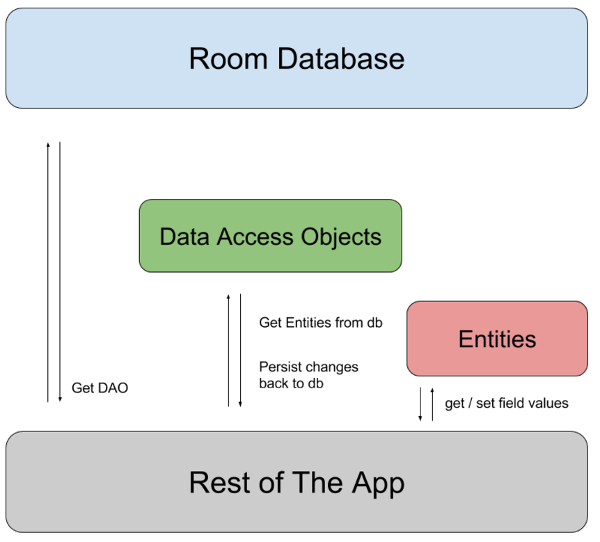
\includegraphics[width=8cm]{images/roomarchitecture.png}
	\caption{Architecture de Room \cite{9}.}
	\label{roomarchitecture}
\end{figure}
%%%%%  REFERENCE %%%%
\section{Librairies utilis�es}

\begin{description}

\item[WeekView] est une librairie qui affiche la vue d'un calendrier. Elle a �t� utile pour l'affichage des �v�nements sur un calendrier, elle impl�mente �galement plusieurs fonctionnalit�s rendant ainsi l'application plus intuitive.

\item[ColorPicker] est comme son nom l'indique, une librairie qui permet de choisir une ou plusieurs couleurs.

\end{description}
Il est � noter que les librairies utilis�es sont libres, open-source, et disponibles sur GitHub. 

\section{Pr�sentation des interfaces}

\subsection{Interface d'accueil}
 Cette premi�re figure pr�sente l'interface d'accueil. C'est la premi�re interface affich�e � l'utilisateur au lancement de l'application. Son principal composant est une vue calendrier qui regroupe les diff�rents �v�nements pr�alablement ajout�s par l'utilisateur. Chaque �v�nement est affich� avec la couleur du calendrier auquel il appartient. Aussi, nous avons un bouton flottant '\+' qui permet d'ajouter des �v�nements, un menu lat�ral pour naviguer entre les diff�rentes activit�s de l'application, et enfin un menu qui ouvre une liste d�roulante pour changer le type du calendrier.


%\begin{figure}[h]
%\centering
%\subfigure[		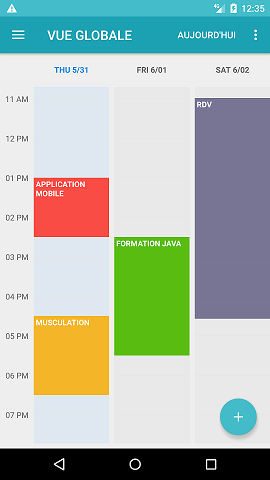
\includegraphics[scale=0.8]{images/homesmall.png}
	%\caption{Interface d'accueil.}
	%\label{home}
%\end{minipage}


\begin{figure}[H]
\centering
	
	\subfigure[Vue Aujourd'hui]{\label{homeaujourdhui}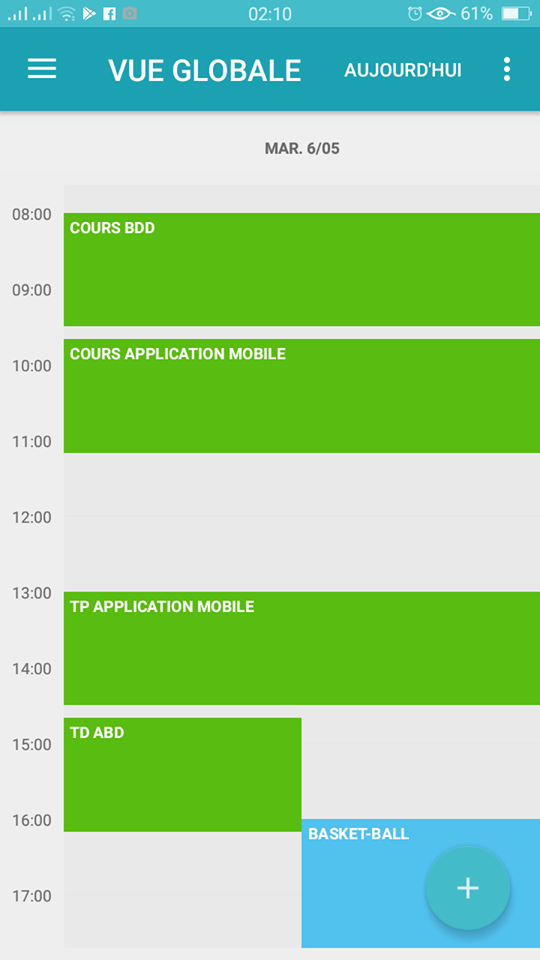
\includegraphics[width=5cm]{images/vue_ajourdui.png}}
	\subfigure[Vue 3 jours]{\label{home3jrs}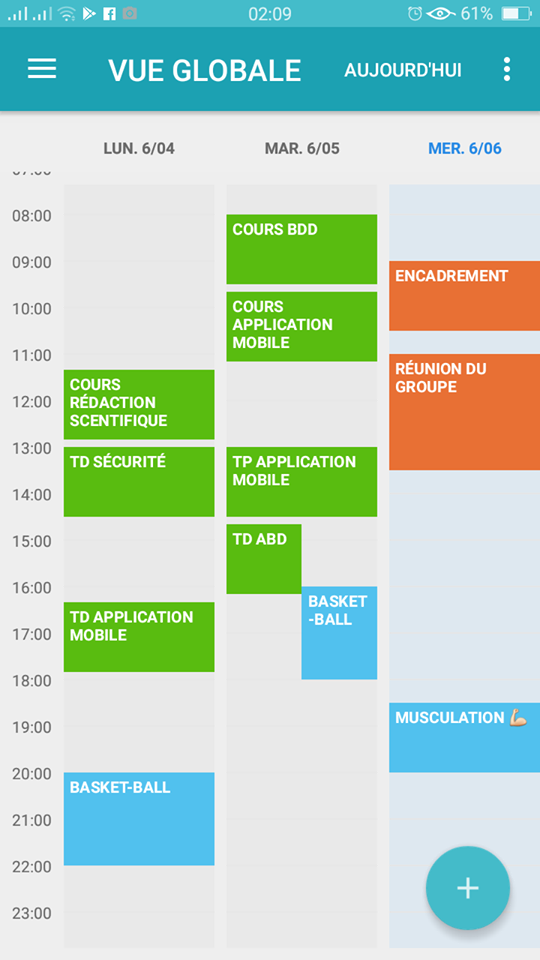
\includegraphics[width=5cm]{images/vue_3jrs.png}}
		\subfigure[Vue une semaine]{\label{home7jrs}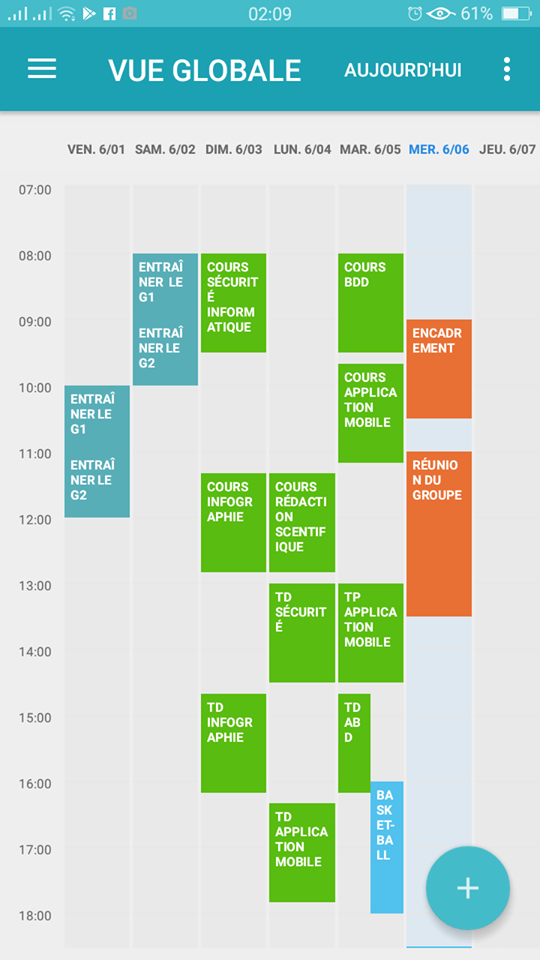
\includegraphics[width=5cm]{images/vue_7jrs.png}}
	\caption{Interface d'accueil}
	\label{home}
	
\end{figure}


\subsection{Interface Calendrier}
La figure \ref{addcalendar} repr�sente la liste des calendriers dont un par d�faut (Mon calendrier) qui est cr�� automatiquement lors de l'installation de l'application. Nous avons �galement d'autres calendriers qui ont �t� ajout�s par l'utilisateur, ces derniers peuvent �tre modifi�s ou supprim�s en appuyant sur le bouton qui lui est associ�. En appuyant sur l'un des calendriers, l'utilisateur est redirig� vers la vue globale contenant seulement les �v�nements qui lui sont affect�s. Pour ajouter un calendrier, il suffit d'appuyer sur le bouton '\+' pour �tre redirig� vers l'interface d'ajout d'un calendrier.  

\begin{figure}[H]
	\centering
		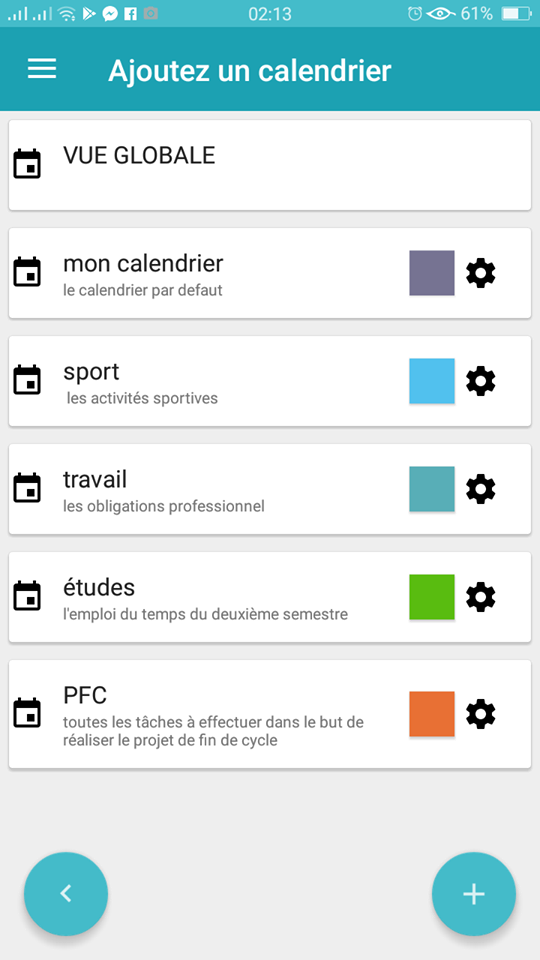
\includegraphics[width=5cm]{images/ajout_calendrier.png}
	\caption{Interface calendrier.}
	\label{addcalendar}
\end{figure}

\subsection{Interface d'ajout d'�v�nement}	

La figure ci-dessous repr�sente l'interface d'ajout d'un �v�nement. L'utilisateur est invit� � remplir les champs, � choisir � quel calendrier appartient-il et enfin � d�cider � quel moment il souhaite �tre alert�, d�sactiver compl�tement l'alerte, sinon.
\begin{figure}[H]
	\centering
		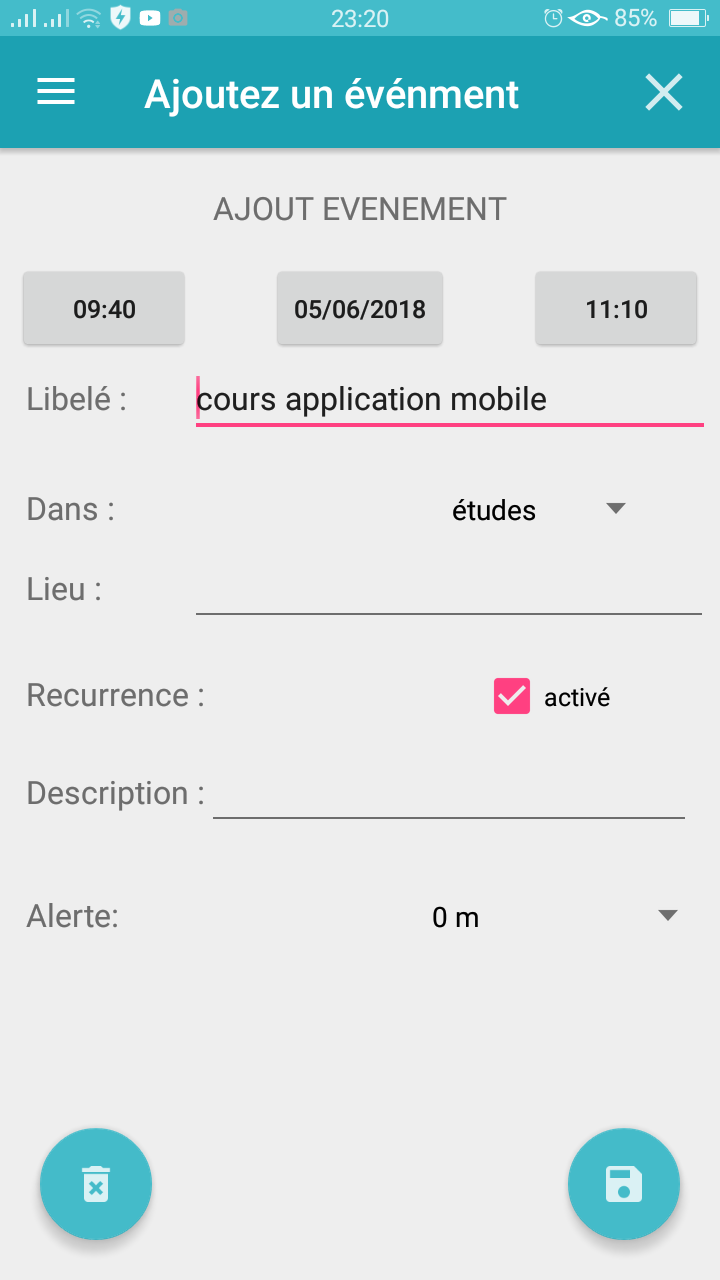
\includegraphics[width=5cm]{images/addevent.png}
	\caption{Ajout d'un �v�nement.}
	\label{addevent}
\end{figure}
\section{Conclusion}

Dans ce dernier chapitre, nous avons revu notre environnement de d�veloppement et d�crit les outils utilis�s notamment GitHub qui a �t� un outil cl� pour notre travail collaboratif. Nous avons �galement vu les diff�rents langages de programmation. Concernant la base de donn�es, Room a �t� un v�ritable atout avec sa facilit� � g�rer et � impl�menter la base de donn�es. Un gain de temps que l'on attribue, aussi, aux diff�rentes librairies. Enfin, nous avons vu les diff�rentes interfaces principales qui composent notre application.

%%%% Conclusion G�n�rale %%%%
\input{Conclusion_G�n�rale}

%%%% Bibliographie %%%%
\begin{thebibliography}{2}
\addcontentsline{toc}{part}{Bibliographie}
		
		
		\bibitem[1]{1} \textsc{ Pascal Roques}, \emph{UML 2 Mod�liser une Application Web}, 4$^e$ �dition, Eyrolles, Paris, 2008.

		\bibitem[2]{2} \textsc{Laurent AUDIBERT},\emph{UML 2 de l'apprentissage a la pratique },Publi� le 31 octobre 2006 - Mis � jour le 12 janvier 2009       ,sur:https://laurent-audibert.developpez.com/Cours-UML/ 
		
		\bibitem[3]{3} \textsc{Laurent Audibert},\emph{UML 2 : de l'apprentissage � la pratique},Ellipse,2$^e$,2009
		
		\bibitem[4]{4}  http://niedercorn.free.fr/iris/iris1/uml/uml10.pdf.
										
		\bibitem[5]{5}	http://www.ai.univ-paris8.fr/~lysop/bd/seance4-ModeleRel.pdf.
		
	  \bibitem[6]{6}	http://tvaira.free.fr/dev/fiches/fiche-c16-diagramme\_classes\_conception.pdf.
		
		
\end{thebibliography}

%%%% R�sum�/Abstract %%%%
\input{R�sum�}

\end{document}